\subsection{Cauchy 判别准则}

设 \((x_{t})_{t\in I}\) 是 \(G\) 中的可和族。那么对每个邻域 \(V\)（\(G\) 中原点的邻域），存在有限子集 \(J_{0}\)（\(I\) 的），使得

对 I 的不与 \(J_{0}\) 相交的每个有限子集 K，都有 \(s_{K} \in V\)。因为 \(J = J_{0} \cup K\) 是包含 \(J_{0}\) 的任意有限子集；设 \(s = \sum x_{i}\)，并设 W 是 o 的对称邻域使得 \(W + W \subset V\)；于是由定义 1，可选取 \(J_{0}\) 使得 \(s_{J} \in s + W\) 且 \(s_{J_{0}} \in s + W\)，这就意味着 \(s_{K} = s_{J} - s_{J_{0}} \in W + W \subset V\)。

反之，设族 \((x_{i})\) 具有这一性质。那么滤子 \(\Phi\) 在映射 \(J \to s_{J}\) 下的像是 G 中的 Cauchy 滤子基。因为若 J 是包含 \(J_{0}\) 的有限子集，且用 K 表示 \(J \cap \complement J_{0}\)，则 \(K \cap J_{0} = \emptyset\) 且 \(s_{K} = s_{J} - s_{J_{0}}\)，于是 \(s_{J} \in s_{J_{0}} + V\)。若 \(J'\) 是包含 \(J_{0}\) 的另一个有限子集，则 \(s_{J} - s_{J'} \in V + V\)，结论由此得出。从而：

定理 1（Cauchy 判别准则）. 在豪斯多夫交换群 G 中，为使族 \((x_{t})_{t\in I}\) 可和，必须对 G 中原点的每个邻域 V，存在 I 的有限子集 \(J_0\)，使得 \(\sum_{i\in K}x_i\in V\) 对 I 的所有不与 \(J_0\) 相交的有限子集 K 成立。若 G 是完备的，这个必要条件也是充分的。

于是，从族 \((x_{i})\) 中去掉（足够多的）有限项后，剩余子族的每个有限部分和都可以任意接近 o。

定理 1 第一部分的一个直接推论是下面的命题：

命题 1. 若族 \((x_{t})\) 可和，则 o 的每个邻域都包含除一个有限子族外的所有 \(x_{t}\)（换句话说，若 I 是无限集，则关于 I 的有限子集的余集所成的滤子，我们有 \(\lim x_{t} = 0\)）。

\pandocbounded{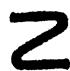
\includegraphics[keepaspectratio]{images/part002_cfff7d82.jpg}}

族 \((x_{i})\) 可和的这一必要条件一般绝不是充分的，即使 \(G\) 是完备的也是如此；后面我们会看到许多例子（见第四章，§ 7）。

推论. 设 \((x_{t})_{t\in I}\) 是交换群中的可和族，且该群的单位元有可数基本邻域系。那么指标 \(\iota\) 中使 \(x_{\iota}\neq 0\) 的那些组成的集合是可数的。

设 \((\mathbf{V}_{n})\) 是 0 的可数基本邻域系。若 \(\mathbf{H}_{n}\) 是使 \(x_{i} \notin \mathbf{V}_{n}\) 的所有指标 i 组成的集合，则使 \(x_{i} \neq 0\) 的指标 i 组成的集合 H 是诸集合 \(\mathbf{H}_{n}\) 的并，而由命题 1，每个 \(\mathbf{H}_{n}\) 都是有限的。

如果我们不假设原点有可数基本邻域系，这个推论就未必再成立。* 例如考虑积群 \(\mathbf{R}^{\mathbb{R}}\){[}实变量的所有有限实值函数作成的加法群，赋以逐点收敛拓扑（参看第十章，§ 1，第 3 节）{]}，并设 \(f_{a}\) 是 \(\mathbf{R}\) 中满足 \(f_{a}(a)=1\) 且 \(f_{a}(x)=0\)（当 \(x\neq a\) 时）的元素；那么族 \((f_{a})_{a\in\mathbb{R}}\) 是可和的，其和是在 \(\mathbf{R}\) 的每点取值都为 1 的函数。 *

注. 当 G 写作乘法时，Cauchy 判别准则取如下形式：为使族 \((x_{i})_{i\in I}\) 可乘，必须对单位元的每个邻域 V，存在 I 的有限子集 \(J_{0}\)，使得对 I 的每个不与 \(J_{0}\) 相交的有限子集 K，都有 \(\prod_{i\in K}x_{i}\in V\)；而且只要 G 是完备的，这个条件也是充分的。由此推出，若 I 是无限集且 \((x_{i})\) 可乘，则关于 I 的有限子集的余集所成的滤子，有 \(\lim x_{i}=1\)；若此外单位元还有可数基本邻域系，则使 \(x_{i}\neq1\) 的指标 i 组成的集合是可数的。

